\chapter{Prolog with Breadth-First Partitioning} 
\label{bfp_depth}

This chapter reviews the performance and behaviour of
some test PrologPF programs, with comparison with DelphiKS, the previous
implementation of the Delphi machine assessed 
by Saraswat in \cite{Sar95}.
Further analysis is given of the breadth-first partitioning strategy used
by PrologPF, particularly of the selection of the depth limit parameter used
in the partitioning phase of execution.

%%%%%%%%%%%%%%%%%%%%%%%%
\section{Introduction} %
%%%%%%%%%%%%%%%%%%%%%%%%
\enlargethispage{-\baselineskip}   % manual final formatting: shorten page by one line

The Breadth-First Partitioning scheduling strategy is described in detail by
Saraswat in his work on DelphiKS
\cite{Sar95} and summarised in Chapter \ref{background} section
\ref{delphi_machine_pwork}.

The execution of the strategy requires that three parameters
are passed to the path processor
with the associated compiled program:
\begin{enumerate}
\item{$G$: the total number of path processors working in parallel}
\item{$N$: the unique processor number assigned to a given path processor}
\item{$L$: the depth bound at which open oracles are recorded in the
  initial search phase, for subsequent allocation for execution}
\end{enumerate}

In \cite{Sar95}, Saraswat analysed a number of benchmarks with several different
strategies with processor group sizes ($G$) from $1$ to
$30$ to assess the efficiency of the speedup of the Delphi machine.
This comparative assessment of PrologPF differs from the approach in
\cite{Sar95}:
\begin{itemize}
\item{While \cite{Sar95} evaluates a variety of strategies, this assessment
  is limited to that found to have the best performance across the range of
  test programs, namely Breadth-First Partitioning.}
\item{Saraswat included a number of benchmarks known to contain little or
  no OR-parallelism.  Evaluation of these benchmarks with DelphiKS confirmed
  the expected absence of parallel speedup.}
\item{This study provides a detailed analysis of the behaviour of the strategy
  with differing values of $L$, rather than the optimal values of $L$ used
  for the runtime versus $G$ graphs in \cite{Sar95}.}
\end{itemize}

%%%%%%%%%%%%%%%%%%%%%%%%%%%
\section{Benchmarks used} %
%%%%%%%%%%%%%%%%%%%%%%%%%%%

The source code for the benchmarks is given in Appendix \ref{benchmarks}. The
appendix also includes graphical representations of the search tree for
each benchmark, with the tree for the 8-queens problem repeated here.

\subsection{8-queens}
%%%%%%%%%%%%

The 8-queens benchmark finds solutions to the problem of placing eight queens on
an  8-by-8 chessboard with no two pieces on the same horizontal, vertical or
diagonal line of squares.  The simple benchmark finds all 92 solutions,
including those which are rotated or reflected versions of other solutions.

The problem has a maximum search depth of 60, and a geometric representation of
the complete search tree is given in Figure \ref{q8_tree}.  The root of the
search tree appears at the top of the figure, and the ``depth'' value
of the ordinate represents the nested depth of subgoals into the search.
The OR-only tree contains a maximum of approxiamtely 1500 open branches at
a depth of 45.

\begin{figure}[htb]
\vspace{5mm} \hbox to \hsize{\hfill \psfig{file={bfp_depth/ps/q8_tree.ps}} \hfill}
\caption{Search tree for 8 queens problem.}
\vspace{5mm}
\label{q8_tree}
\end{figure}

The other benchmarks have much larger search trees than the 8 queens problem.
The complete mapping of
the search space resulting in the tree diagram in Figure \ref{q8_tree} has not been
repeated here for the other benchmarks, but are in Appendix \ref{benchmarks}.

\subsection{10-queens}
%%%%%%%%%%%%

This benchmark is identical to the 8-queens benchmark described above, except
the problem is extended to place ten queens on a 10-by-10 chessboard.

The problem has 724 solutions, and the
maximum depth of the search tree is 85.  The OR-only tree has a maximum of
approximately 26000 branches at a depth of 65.


\subsection{Pentominoes}
%%%%%%%%%%%%

A pentomino is a shape made up of five equal-sized squares, for example in the
shape of a letter \texttt{T} or a letter \texttt{L}.
There are twelve possible shapes from five connected squares, and the
 benchmark program
\texttt{pentbook} attempts to fit these pieces on a 20-by-3 board.
Each piece has a number of possible orientations and reflections, and 
can be used only once. The
benchmark finds 8 solutions.
The maximum depth of the search tree is 90, with the maximum of approximately
100,000 branches open at a depth of 58.
The Prolog source for the benchmark \texttt{pentbook} is contained in 
Appendix \ref{pent_benchmark}.

\subsection{Other benchmarks in DelphiKS}
%%%%%%%%%%%%

In addition to the benchmarks discussed above, Saraswat in \cite{Sar95}
analysed a
number of additional programs which have not been included in this comparison:
\begin{description}
\item[FFT:]{ a fast-Fourier transform algorithm which contains no
  OR-parallelism, and thus showed no speedup on the Delphi machine.  Similarly,
  no speedup would be expected with the use of PrologPF.}
\item[Adder, Permutation, Balanced:]{ these benchmarks have low runtimes
  even with a single cpu, and some generate many solutions.  For example, the
  \texttt{perm} benchmark compiled with the PrologPF compiler completes in
  540 milliseconds on a single cpu, generating 720 solutions.
  The short runtime and large
  number of solutions cause the input/output requirements to dominate the
  execution times in any attempt at parallel speedup.
  DelphiKS took
  7.87 seconds to execute the \texttt{perm} benchmark on the same single
  processor, with more scope for parallel improvement. The \texttt{adder}
  and \texttt{balanced} benchmarks took 12.61 seconds and 6.23 seconds
  to execute on a single cpu DelphiKS system respectively.}
\end{description}


\section{Implementation differences}
%%%%%%%%%%%%

\subsection{DelphiKS}
%%%%%%%%%%%%%%%

The previous implementation of the Delphi machine, DelphiKS \cite{Kle91,Sar95}
included support for additional WAM \cite{War83} instructions:
\begin{description}
\item[onumtry, onumretry, onumtrust:]{ these DelphiKS instructions are analogous
  to their WAM counterparts \cite{AK90}, building and removing choice points at the
  entry-points of compiled alternative clauses in nondeterministic procedures.  The
  DelphiKS instructions accumulate the current oracle as the search proceeds, and
  provide support for following oracles when executing in that mode.}
\item[onumsing:]{ this is a special instruction placed at the entry point of the
  clause where a procedure contains only a single clause, such that no choice
  point is built and the current oracle need not be extended.  The instruction
  is used instead of the usual nondeterministic instructions listed above when
  non-backtracking strategies are used.}
\item[setmax:]{ this instruction is inserted at the beginning of each procedure,
  before the first clause.  It provides a point at which the number of alternative
  clauses in the procedure can be recorded.  This information can be used to
  determine the right number of bits to remove from the binary oracle being
  followed.  The \texttt{setmax} instruction provides the point at which
  scheduling decisions can be taken in the path processor.  For example, as
  the number of alternatives is known at this point (in the argument to
  \texttt{setmax}) the incremental extensions to the current oracle can be built
  and returned to the control processor.  Alternatively the current depth can
  be checked against the depth bound in the breadth-first partitioning
  strategy.}
\end{description}

In addition to the extra instructions, the extended WAM maintains a
few data structures, most notably the oracle stack.

\subsection{Prototype PrologPF with Prolog oracles}
%%%%%%%%%%%%%%%

In this implementation of PrologPF the user program is transformed to a 
version in which every relation has additional arguments, such that the
current oracle is propagated through the procedure calls.  The Prolog
support for difference lists and logical variables is exploited for an
efficient implementation.

A utility procedure \texttt{o\_{}next(N,A)} is provided which returns the next
choice index of the current oracle in \texttt{N} and accepts the current oracle
\texttt{A} as an argument.  If the program is being used to \textbf{build} an
oracle then \texttt{N} will be returned as a logical 
variable embedded in \texttt{A}, such
that the immediately following call of a relation will instantiate that variable
to the clause index.
For example, the following program illustrates the transformation:
\begin{alltt}
  a(X) :- b(X), c(X).\vspace{2mm}
  b(a).
  b(c).\vspace{2mm}
  c(c).
\end{alltt}
this is transformed to:
\begin{alltt}
  a(1,A,[1|E],En,X) :- o_next(N1,A), b(N1,A,E,En,X),
                       o_next(N2,A), c(N2,A,E,En,X).\vspace{2mm}
  b(1,A,[1|E],E,a).
  b(2,A,[2|E],E,c).\vspace{2mm}
  c(1,A,[1|E],E,c).
\end{alltt}

A query such as \texttt{a(X)} is replaced with \texttt{o\_{}next(N,A),a(N,A,A,X)} in
which \texttt{o\_{}next(N,A)} provides the first oracle element \texttt{N}
to be used as the first argument of the goal, and \texttt{A,A} represents the
empty difference list of the initial oracle.

An oracle to be followed is stored as a Prolog list in a global variable.

The general format of each relation is:\\
\centerline{\texttt{relation\_{}name(cn, orc, orc\_{}hole, new\_{}hole, args\ldots)}}
where:
\begin{description}
\item[\texttt{cn}:]{ clause number, in textual sequence of procedure.}
\item[\texttt{orc}:]{ oracle accumulated so far and passed to procedure as
  difference list.}
\item[\texttt{orc\_{}hole}:]{ logical variable representing end of \texttt{orc}.}
\item[\texttt{new\_{}hole}:]{ variable returned by procedure as new hole at end
  of extended \texttt{orc} when the procedure succeeds.}
\end{description}
The semantics of \texttt{o\_{}next(N,A)} are:\\
on first call:\\
\begin{tabular}{l l l}
\texttt{o\_{}next(N,A)} & :- & \textit{if (current mode = FOLLOWING an oracle)}\\
                        &    & \textit{then N := next oracle element}\\
                        &    & \textit{else /* currently BUILDING an oracle */}\\
                        &    & \textit{~~~~if (current depth = depth limit L)}\\
                        &    & \textit{~~~~then}\\
                        &    & \textit{~~~~~~~~push A onto oracle stack;}\\
                        &    & \textit{~~~~~~~~}\texttt{fail}\\
                        &    & \textit{~~~~else}\\
                        &    & \textit{~~~~~~~~increment current depth.}
\end{tabular}

and on backtracking:\\
\begin{tabular}{l l l}
\texttt{o\_{}next(\_{},\_{})} & :- & \textit{decrement current depth,}\\
                              &    & \texttt{fail.}
\end{tabular}

At any point during the execution of the program, the logical variable
\texttt{A} contains the current oracle.
The implementation of oracle support using Prolog procedures and
data structures provides a flexible tool for
the analysis of different strategies, but generates considerable overhead.

\subsection{PrologPF with C oracles}
%%%%%%%%%%%%%%%
\label{c_macros}

To reduce the overhead of the use of Prolog data structures to represent
oracles and the definition of the utility relations such as \texttt{o\_{}next} as
Prolog procedures, the oracle support in PrologPF was re-implemented in C.

For simplicity of implementation and debugging, a similar program
transformation technique was used, but with more efficient primitives.
As an example of the more efficient transformation, the same example will
be used as above.
\begin{alltt}
a(X) :- b(X), c(X).\vspace{2mm}
b(a).
b(c).\vspace{2mm}
c(c).
\end{alltt}
The user program can be transformed into two subprograms, one suitable for
building an oracle as the search progresses, and the other suitable for
following an assigned oracle.

As the execution progresses, to accumulate an oracle as the search tree is traversed the
sample program can be transformed by the compiler to:
\begin{alltt}
% BUILD code \vspace{2mm}
a(X) :- o_build(1), b(X), c(X).\vspace{2mm}
b(a) :- o_build(1).
b(c) :- o_build(2).\vspace{2mm}
c(c) :- o_build(1).
\end{alltt}

The special relation \texttt{o\_{}build} is defined as follows:\\

\texttt{o\_{}build(X) :- }\textit{append index $X$ to end of current oracle.}\\
\texttt{o\_{}build(\_{}) :- }\textit{pop last index from oracle,}\texttt{ fail.}

The \texttt{o\_{}build} relation is defined using C macros, and has the side-effect of
updating the state of the current oracle.  At any point in the search, the current oracle
represents the sequence of clause indexes to traverse the tree directly to the current
node.

A query such as \texttt{:- a(X)} will initially create an oracle \textit{[1]}, and then
solve the subgoal \texttt{b(X)}, appending \textit{1} to the current oracle and returning
with the solution \{\texttt{X/a}\}.  Then the subgoal \texttt{c(a)} is called, which fails,
and on backtracking the \texttt{b(X)} goal removes the appended \textit{1} from the oracle
and searches for an alternative solution for \texttt{b(X)}.  The \texttt{b(c)} clause is
tried and succeeds, appending \textit{2} to the current oracle and returning the solution
\{\texttt{X/c}\}.  The subgoal \texttt{c(c)} is now called, appending \textit{1} to the 
current oracle and succeeding.  The \texttt{a(X)} goal succeeds, at which point the current
oracle is \textit{[1,2,1]}.

For the purposes of strategies such as breadth-first partitioning, it is useful to
accumulate additional state information as the search progresses, particularly the
current depth of the search, or equally the length of the current oracle.  Breadth-first
partitioning requires the use of a depth limit (referred to as $L$).  To constrain the
search to within this depth, the \texttt{o\_{}build} relation can be made to \textit{fail}
whenever this depth is reached.  So the extended definition of \texttt{o\_{}build} is as
follows, with the depth initially zero:

\begin{tabular}{l l l}
\texttt{o\_{}build(X)}    & :- & \textit{increment depth}\\
                          &    & \textit{append index $X$ to end of current oracle.}\\
                          &    & \textit{if depth = $L$}\\
                          &    & \textit{then record current oracle and }\texttt{fail.}\\
\texttt{o\_{}build(\_{})} & :- & \textit{decrement depth}\\
                          &    & \textit{pop last index from oracle}\\
                          &    & \texttt{fail.}\\
\end{tabular}

The pseudo-code for \texttt{o\_{}build} show it has the following characteristics:
\begin{itemize}
\item{the first clause succeeds if the current depth is not equal to $L$}
\item{the second clause always fails}
\item{if the current depth is less than $L$, the relation always has one solution}
\item{if the current depth is equal to $L$, the relation always fails}
\item{the current depth can never become greater than $L$}
\item{when the query completes the depth will be zero, as each increment operation is
  always followed by an associated decrement.}
\end{itemize}

In the implementation in PrologPF, the current oracle is accumulated in a C array with
the current depth as the index.

It should be noted that the \textit{build} code described above records the oracles at
points in the search where the current depth equals the depth limit $L$.  In order to
\textit{follow} these open oracles, a different transformation of the sample program
can be used:
\begin{alltt}
% FOLLOW code\vspace{2mm}
a(1,X) :- o_follow(N1), b(N1,X), o_follow(N2), c(N2,X).\vspace{2mm}
b(1,a).
b(2,c).\vspace{2mm}
c(1,c).
\end{alltt}
A query such as \texttt{a(X)} will similarly be transformed to \texttt{o\_{}follow(N), a(N,X)}.
Given an oracle built by the transformed program using \texttt{o\_{}build} described earlier, the
definition of the special relation \texttt{o\_{}follow} is as follows:\\
\begin{tabular}{l l l}
\texttt{o\_{}follow(X)}   & :- & \textit{return with X = next index from current oracle.}
\end{tabular}

This definition of \texttt{o\_{}follow} is satisfactory when the oracle being followed leads
directly to a solution (or failure).  If the assigned oracle is in fact \textit{open}, i.e. leads
to an intermediate node in the search tree, then additional support is required.  After following an
open oracle to its end, PrologPF will then continue the search in \texttt{build} mode.  This can
be viewed as generating extensions to the supplied current oracle.  This cross-over from the
transformed program providing oracle following support to the code to build the oracle extension
can be achieved by extending the program transformation with additional clauses:
\begin{alltt}
% FOLLOW code\vspace{2mm}
a(1,X) :- o_follow(N1), b(N1,X), o_follow(N2), c(N2,X).
a(0,X) :- a(X).  % crossover clause\vspace{2mm}
b(1,a).
b(2,c).
b(0,X) :- b(X).  % crossover clause\vspace{2mm}
c(1,c).
c(0,X) :- c(X).  % crossover clause
\end{alltt}
The \texttt{o\_{}follow} relation is similarly extended to return \textit{0} as an index
when it reaches the end of the currently followed oracle.  From this point on, all subgoals will
map to their \textit{build} counterparts and the search can continue, again using a depth limit
if required.

With the breadth-first partitioning strategy the unconstrained search in the
second phase means the overhead of the accumulation of the current oracle in
that phase is unnecessary.  The \textit{crossover} clause could equally
transfer execution to the subprogram with no oracle support, for an
execution efficiency identical to that of the standard Prolog compiler.
However, more complex strategies, particularly those requiring
redistribution of work during the second phase, would require the continued
accumulation of the current oracle.

As with the \texttt{o\_{}build} relation, the \texttt{o\_{}follow} relation maintains a global value
to represent the current depth in the search.  This depth is also the index into the C array 
containing the current oracle.

In the \textit{follow} transformation described above, the oracle index has been shown as an 
new first parameter added to the head of each clause.  The indexing of the first argument used in
most Prologs and the C macro implementation of \texttt{o\_{}follow} means the following of oracles
can be particularly efficient.

The transformations of the sample program into the \textit{build} code and \textit{follow} code
results in a program suitable for executing many scheduling strategies with small adjustments to
the definitions of \texttt{o\_{}build} and \texttt{o\_{}follow}.
The transformations described above are applicable to all implementations of Prolog providing
linkage to C routines or macros.

In PrologPF, a small trade-off has been made against execution efficiency for a simpler combined
transformation, retaining the use of \texttt{o\_{}build} and \texttt{o\_{}follow}.  The transformed
program in PrologPF is considered to execute in one of two modes, \textit{build} or
\textit{follow}, such that the \texttt{o\_{}build} and \texttt{o\_{}follow} relations behave as
before in the \textit{build} and \textit{follow} modes respectively, otherwise they do nothing.
The combined transformation used in PrologPF is as follows:
\begin{alltt}
a(X,1) :- o_build(1), o_follow(N1), b(X,N1), o_follow(N2), c(X,N2).\vspace{2mm}
b(a,1) :- o_build(1).
b(c,2) :- o_build(2).\vspace{2mm}
c(c,1) :- o_build(1).
\end{alltt}

An associated query such as \texttt{a(X)} is similarly transformed to:\\
\centerline{\texttt{o\_{}follow(N),A(X,N)}.}

The added clause index is moved to the end of the parameter list in the head of each clause, so that
Prolog indexing on the first parameter can still be exploited in \textit{build} mode.  The
breadth-first partitioning strategy is designed to involve much more search (in build mode) than the
initial following of assigned oracles by path processors, so the indexing of the added arguments 
in the implementation described previously has been
forfeited.

\subsection{BFP and oracle allocation algorithm}
%%%%%%%%%%%%%
\label{oracle_alloc}

The implementation of the breadth-first partitioning strategy is the same for
the oracle support in C or Prolog:
\begin{enumerate}
\item{The arguments $G$, $N$ and $L$ are read from the command line.}
\item{The depth limit is set to $L$ and a \textit{build} version of the
  query is called.  This results in a stack of oracles in the global array.}
\item{Beginning with the $N$th oracle, and subsequently with every $G$th
  oracle, the path processor executes a \textit{follow} version of the
  query with the depth limit $L=\infty$. 
  I.e.~path processor $N$ will be allocated the $i$th oracle
  iff $(i$ mod $G) = N$. Solutions found are reported to
  the control processor.}
\item{Completion is reported to the control processor.}
\end{enumerate}

%%%%%%%%%%%%%%%%%%%%%%%%%%%%%%%%%%
\section{Single CPU performance} %
%%%%%%%%%%%%%%%%%%%%%%%%%%%%%%%%%%

The Prolog programs compiled for the Delphi Machine and with the PrologPF
compiler can be successfully run on a system with a single cpu simply by
specifying the group size $G=1$, and allocating the selected processor the
unique processor number $0$.  The execution performance of the Delphi
implementations can then be compared with each other and with some
sequential implementations of Prolog to assess the overhead caused by the
use of oracles.

\subsection{Single CPU comparison: DelphiKS, PrologPF, sequential Prolog}
%%%%%%%%%%%%

The bar charts in figures \ref{single_cpu_queens8}, \ref{single_cpu_queens10}
and \ref{single_cpu_pentbook} compare the performance of the following
systems using a single processor\footnote{MIPS-based DECStation 3100}:
\begin{description}
\item[DelphiKS:]{ the figures for the single cpu performance of the
  previous implementation of the Delphi machine by Klein \cite{Kle91} are taken
  from Saraswat's analysis \cite{Sar95}.}
\item[PrologPF:]{ these figures refer to the execution of the compiled
  benchmarks using the prototype implementation of PrologPF using Prolog
  data structures to hold the oracles, and Prolog procedures to build and
  follow oracles.}
\item[PrologPF(C):]{ these figures are from the benchmarks compiled
  with the runtime oracle support in PrologPF implemented as C macros
  (see section \ref{c_macros}).}
\item[wamcc:]{ the benchmarks were compiled with the sequential Prolog
  compiler \texttt{wamcc} on which PrologPF is based, and runtimes from
  a single processor were recorded.}
\item[Sicstus:]{ the SICStus sequential Prolog compiler
  (SICStus Version 3 \cite{BBP+94})
  was used to produce a \textit{compactcode} compiled file, for loading and
  executing with the SICStus runtime system.  The compiler option producing
  the fastest binaries,
  \textit{fastcode}, was not available for the MIPS systems used in the
  test.}
\end{description}

As the scheduling strategy is of no purpose
in a single cpu environment, the overhead of the 
breadth-first partitioning strategy was minimised by setting the depth
limit $L=1$.  The compiled files produced by PrologPF thus spent very little
time in the initial partitioning phase (less than 1ms), and the overhead of
PrologPF versus wamcc is caused by the runtime management of the current
oracle during the progress of the search.
\begin{figure}[htb]
\vspace{5mm} \hbox to \hsize{\hfill \psfig{file={bfp_depth/ps/single_cpu_queens8.ps}} \hfill}
\caption{Single cpu runtimes for 8-queens benchmark.}
\vspace{5mm}
\label{single_cpu_queens8}
\end{figure}

\begin{figure}[htb]
\vspace{5mm} \hbox to \hsize{\hfill \psfig{file={bfp_depth/ps/single_cpu_queens10.ps}} \hfill}
\caption{Single cpu runtimes for 10-queens benchmark.}
\vspace{5mm}
\label{single_cpu_queens10}
\end{figure}

\begin{figure}[htb]
\vspace{5mm} \hbox to \hsize{\hfill \psfig{file={bfp_depth/ps/single_cpu_pentbook.ps}} \hfill}
\caption{Single cpu performance for Pentominoes benchmark.}
\vspace{5mm}
\label{single_cpu_pentbook}
\end{figure}

The single processor execution times for each benchmark with each compiler 
are given in Table \ref{single_cpu_table}.

\begin{table}[htb]
{\small
\begin{tabular}{| l | r | r | r | r | r |}
\hline
 & & & & & \\[2mm]
\textbf{Benchmark} & \textbf{DelphiKS} & \textbf{PrologPF(Prolog)} & \textbf{PrologPF(C)} & \textbf{wamcc} & \textbf{SICStus} \\
\hline
\textbf{8-queens} & 59780 & 7859 & 1898 & 1636 & 3480 \\
\hline
\textbf{10-queens} & 1198770 & 197956 & 46497 & 38978 & 91490 \\
\hline
\textbf{Pentominoes} & 2824670 & 1041660 & 445959 & 410908 & 340885 \\
\hline
\end{tabular}
}
\caption{Single cpu execution times (in milliseconds)}
\label{single_cpu_table}
\end{table}

The overhead of the oracle support coded with C macros in PrologPF(C)
for each of the three sample benchmarks is given in Table \ref{prologpf_overhead}.

\begin{table}[htb]
{\small
\begin{tabular}{| l | r |}
\hline
\textbf{Benchmark} & \textbf{PrologPF(C) overhead}\\
\hline
8-queens & 16\% \\
\hline
10-queens & 19\% \\
\hline
Pentominoes & 9\% \\
\hline
\end{tabular}
}
\caption{Overhead of PrologPF(C) oracle support.}
\label{prologpf_overhead}
\end{table}

%%%%%%%%%%%%%%%%%%%%%%%%%%%%%%%%%%%%%%%%%%
\section{Parallel execution performance} %
%%%%%%%%%%%%%%%%%%%%%%%%%%%%%%%%%%%%%%%%%%

The runtime and speedup figures for the parallel execution of each benchmark are summarised
in Table \ref{parallel_perf}.

\begin{sidewaystable}
{\small
\begin{tabular}{||l|c|c|c|c|c|c|c|c|c|c|c|c|c|c|c||} \hline
 & \multicolumn{11}{c|}{} & & &  & \\
 & \multicolumn{11}{c|}{ Total Execution Time (with increasing number of path-processors) }                          & Re-   &      & Partit-& Recor- \\
 & \multicolumn{11}{c|}{}                                                                                            & comp. & Ans- & ioning & ded    \\
  \cline{2-12} Test Program & 1     & 3     & 6     & 9     & 12    & 15    & 18    & 21    & 24    & 27    & 30     & Time  & wers & depth  & oracles\\
  \cline{1-16} 8-Queens     & 1.90  & 0.753 & 0.461 & 0.297 & 0.258 & 0.215 & 0.207 & 0.176 & 0.160 & 0.156 & 0.141  & 0.030 &  92  & 21     & 184  \\
  \cline{1-16} 10-Queens    & 46.50 & 15.88 & 8.925 & 5.886 & 5.070 & 3.863 & 3.379 & 3.485 & 3.121 & 2.472 & 2.519  & 0.168 & 724  & 27     & 864   \\
  \cline{1-16} Pentominoes  & 446.0 & 185.0 & 122.7 & 83.02 & 93.22 & 71.27 & 44.69 & 40.83 & 51.39 & 37.26 & 41.49  & 0.672 &   8  & 21     & 848 \\
\hline
 & \multicolumn{11}{c|}{} & & & & \\
 & \multicolumn{11}{c|}{ Speedup factors (with increasing number of path-processors) } & & & & \\
 & \multicolumn{11}{c|}{} & & & &  \\
  \cline{1-16} 8-Queens    & 1      & 2.52  & 4.12  & 6.39  & 7.35  & 8.83  & 9.17  & 10.78 & 11.86 & 12.17 & 13.46  & 0.030 &  92  & 21     & 184  \\
  \cline{1-16} 10-Queens   & 1      & 2.93  & 5.21  & 7.90  & 9.17  & 12.04 & 13.76 & 13.34 & 14.90 & 18.81 & 18.45  & 0.168 & 724  & 27     & 864   \\
  \cline{1-16} Pentominoes & 1      & 2.41  & 3.63  & 5.37  & 4.78  & 6.26  & 9.98  & 10.92 & 8.68  & 11.97 & 10.75  & 0.672 &   8  & 21     & 848 \\
\hline
\end{tabular}
\caption[Parallel execution performance of PrologPF]{Parallel execution
                            performance of PrologPF for
                            appropriate partitioning-depths.}
\label{parallel_perf}
}
\end{sidewaystable}

\subsection{8-queens}
%%%%%%%%%%%%

The graph showing the reduction in runtime for increasing number of 
path processors with a suitable partitioning depth is given in Figure \ref{queens8_cut_c_L_21}.

\begin{figure}[htb]
\vspace{5mm} \hbox to \hsize{\hfill \psfig{file={bfp_depth/ps/queens8_cut_c_L_21.ps}} \hfill}
\caption{Runtimes for 8-queens benchmark for $G=1\ldots 30$ and $L=21$.}
\vspace{5mm}
\label{queens8_cut_c_L_21}
\end{figure}

With the selected depth limit $L=21$ for the breadth-first
partitioning, the program shows consistently reducing runtimes as the
number of path-processors increases from 1 to 30.  The 8-queens
problem has a well balanced search tree, and is therefore suited to
the one-time breadth-first partitioning OR-parallel execution technique used in PrologPF.
The graph of runtime ratios representing
speedups over the single-cpu case are given in Figure \ref{q8_cut_c_L_21_spdup}.

\begin{figure}[htb]
\vspace{5mm} \hbox to \hsize{\hfill \psfig{file={bfp_depth/ps/q8_cut_c_L_21_spdup.ps}} \hfill}
\caption{Speedup for 8-queens benchmark for $G=1\ldots 30$ and $L=21$.}
\vspace{5mm}
\label{q8_cut_c_L_21_spdup}
\end{figure}

As with the runtime graph, the speedup graph shows that with groups of
path-processors in the range $G=1\ldots 30$ there is an improvement in
performance as processors are added.  As will be seen with later
benchmarks, the speedup curve illustrates any reduction in efficiency
as processors are added more clearly than the equivalent runtime
graph.  While the speedup curve for the 8-queens benchmark is
monotonically increasing, it does not increase directly with the
number of available processors $G$.  For example the speedup for
$G=24$ is approximately $12$, so 50\% of the available processing
resource has been effectively applied to the problem.

There are several factors which limit the efficiency of the parallel
execution of the problem, and these are discussed in detail in section
\ref{bfp_issues}.

\subsection{10-queens}
%%%%%%%%%%%%

The graph showing the reduction in runtime for increasing number of 
path processors is given in Figure \ref{queens10_cut_c_L_27};  the reciprocal data representing
speedups over the single-cpu case is given in the graph of Figure \ref{q10_cut_c_L_27_spdup}.
As with the 8-queens benchmark, a suitable value for the depth limit $L$ has been selected for this
initial performance analysis.  The issue of the selection of the depth limit is discussed further in
section \ref{bfp_issues}.

\begin{figure}[htb]
\vspace{5mm} \hbox to \hsize{\hfill \psfig{file={bfp_depth/ps/queens10_cut_c_L_27.ps}} \hfill}
\caption{Runtimes for 10-queens benchmark for $G=1\ldots 30$ and $L=27$.}
\vspace{5mm}
\label{queens10_cut_c_L_27}
\end{figure}

The speedup graph in Figure \ref{q10_cut_c_L_27_spdup} shows a maximum speedup of
approximately $19$ for
any number of path-processors from $G=1\ldots 30$. For two values of $G$, $G=21$
and $G=30$ the speedup is actually less than can be achieved with fewer processors. 
The depth limit $L$ is fixed
at $L=27$ for the parallel execution with each value of $G$, such that the number of oracles
remains fixed at $S=864$.  The variation in speedup arises from the different allocation of 
oracles to path-processors with the simple modular algorithm used in PrologPF.  This issue is 
discussed further in section \ref{bfp_issues}.

\begin{figure}[htb]
\vspace{5mm} \hbox to \hsize{\hfill \psfig{file={bfp_depth/ps/q10_cut_c_L_27_spdup.ps}} \hfill}
\caption{Speedup for 10-queens benchmark for $G=1\ldots 30$ and $L=27$.}
\vspace{5mm}
\label{q10_cut_c_L_27_spdup}
\end{figure}


\subsection{Pentominoes}
%%%%%%%%%%%%

The graph showing the reduction in runtime for increasing number of 
path processors is given in \ref{pentbook_cut_c_L_21},
and the reciprocal data representing
speedups over the single-cpu case in Figure \ref{pent_cut_c_L_21_spdup}.

\begin{figure}[htb]
\vspace{5mm} \hbox to \hsize{\hfill \psfig{file={bfp_depth/ps/pentbook_cut_c_L_21.ps}} \hfill}
\caption{Runtimes for Pentominoes benchmark for $G=1\ldots 30$ and $L=21$.}
\vspace{5mm}
\label{pentbook_cut_c_L_21}
\end{figure}

While showing improvements in runtimes up to approximately 18
path-processors, further increase in $G$ does not result in a
reduction of the runtime below approximately 40 seconds.  At the depth
limit $L=21$ used in the test there are 848 oracles, and one of those
oracles has sufficient work beneath it to cause the associated path
processor to determine the overall runtime figure.  This issue arises
because:
\begin{itemize}
\item{The breadth-first partitioning strategy used in PrologPF
  performs a one-time allocation of oracles without subsequent
  work-splitting.  The introduction of work-splitting with PrologPF
  is described in Chapter \ref{sok}.}
\item{The overall runtime of the parallel execution of the problem is determined by
  whichever path processor takes the longest time to search the subtrees of its
  allocated oracles.}
\end{itemize}
The issue of the presence of large outlying oracles
is discussed further in section \ref{bfp_issues}.

\begin{figure}[htb]
\vspace{5mm} \hbox to \hsize{\hfill \psfig{file={bfp_depth/ps/pent_cut_c_L_21_spdup.ps}} \hfill}
\caption{Speedup for Pentominoes benchmark for $G=1\ldots 30$ and $L=21$.}
\vspace{5mm}
\label{pent_cut_c_L_21_spdup}
\end{figure}

The speedup graph in Figure \ref{pent_cut_c_L_21_spdup} emphasises the limit of reduction
in runtime as a maximum speedup for $L=21$ of 12.  In the same graph, the values of $G$
for which the speedup is actually \textit{lower} than for a run with fewer path-processors
can be seen ($G=12,24 \mbox{ and } 30$).  As with the 10-queens benchmark, these anomalies
arise from the allocation of the 848 oracles at $L=21$ modulo $G$ to the path-processors
(see section \ref{oracle_alloc}).

\subsection{Summary}
%%%%%%%%%%%%

For the benchmarks containing available OR-parallelism tested, PrologPF provides
effective speedup over the single-cpu case.  The parallel computing environment
consists of commonly available workstations interconnected in a typical Ethernet-based
intranet.  With the one-time partitioning of BFP, 
no communication is required between the cooperating processors after the
initial assignment of the work except to return solutions and report completion.

The parallel speedup provided by PrologPF is limited by a number of factors, including:
\begin{itemize}
\item{The size of the problem}
\item{The modular allocation of the open oracles}
\item{The one-time allocation of the open oracles, without subsequent work-splitting}
\end{itemize}

These issues are discussed in detail in the remainder of this chapter.

%%%%%%%%%%%%%%%%%%
\section{Issues} %
%%%%%%%%%%%%%%%%%%
\label{bfp_issues}

The performance tests from the three benchmark programs highlighted three issues
affecting the maximum speedup available with PrologPF:
\begin{itemize}
\item{Although the problems with available OR-parallelism show a speedup with increasing
  numbers of path-processors, the slope of the speedup graph is less than 1.  An ideal
  parallel implementation with $G$ processors would achieve a speedup of $G$, and
  PrologPF falls short of this goal, sometimes dramatically.}
\item{For some values of $G$ the speedup with a given depth limit $L$ is \textit{less} than
  the speedup with fewer path-processors.}
\item{At some value of $G$ for a given depth limit $L$, the runtime of the parallel
  execution of the problem reaches a lower limit, after which no improvement in runtime
  is available with increasing $G$.}
\end{itemize}

These issues are apparent even with an optimally selected value of $L$.  The causes are
as follows:
\begin{enumerate}
\item{The initial phase of the breadth-first partitioning scheduling 
  strategy, producing open oracles at the depth limit $L$, is performed sequentially
  before the subsequent allocation of the discovered oracles to path processors.  The
  time taken for this initial phase places an upper bound on the speedup possible.
  This problem is most significant for problems with relatively small search trees.}
\item{PrologPF uses a simple modular allocation algorithm, given in section
  \ref{oracle_alloc}, to allocate the discovered oracles to the $G$ available path
  processors.  No estimate is made of the size of the subtree below each oracle before
  it is assigned to a path processor.  Some values of $G$ may cause the distribution
  of the oracles to be particularly unfavourable.
  As the parallel runtime with one-time partitioning 
  is dependent on the maximum runtime of any
  contributing path processor, a bad distribution of oracles can
  result in a runtime worse than
  that of a more favourable distribution on fewer path processors.}
\item{With a selected value of the depth limit $L$, a fixed number of open oracles
  is produced.  As PrologPF with one-time partitioning
  performs no work splitting after the initial assignment
  of an oracle, the parallel speedup is limited by the runtime of the search of the
  largest subtree.}
\end{enumerate}

\subsection{Oracle discovery and allocation}
%%%%%%%%%%%%
\label{orc_discovery}

In its first phase of execution of the 8-queens problem, PrologPF
 performs sequential computation for an average of $30$ milliseconds to
 produce the $184$ open oracles at the depth limit $L=21$ (see Table
 \ref{parallel_perf}).
The single-cpu execution of the 8-queens problem completes in $1898$ milliseconds (Table
\ref{single_cpu_table}).  The overhead of the initial breadth-first phases places an
upper bound of $1898/30$, or $63$, on the possible speedup for $L=21$.

The $184$ open oracles discovered at $L=21$ reference subtrees containing varying amounts
of work.  The distribution of the work expressed in milliseconds per oracle is given
in Table \ref{q8_orcs}.

\begin{table}[htb]
{\small
\begin{tabular}{| l | r @{} r @{} r @{} r @{} r @{} r @{} r @{} r @{}
    r @{} r @{} r @{} r @{} r @{} r @{} r @{} r @{} r @{} r @{} r @{} 
    r @{} r @{} r @{} r @{} r @{} r |}
\hline
\textbf{Work (ms):} & 0 & & 5 & & 10 & & 15 & & 20 & & 25 & & 30 & & 35 & & 40
     & & 45 & & 50 & & 55 & & 60 \\
\hline
\textbf{Oracles:} & & 65 & & 27 & & 32 & & 37 & & 6 & & 7 & & 8 & & 1
   & & 0 & & 0 & & 0 & & 1 &\\
\hline
\end{tabular}
}
\caption{Oracle work distribution for 8-queens at $L=21$}
\label{q8_orcs}
\end{table}

With the one-time allocation of oracles on the completion of the first phase of
the breadth-first partitioning strategy, with $G=30$ each path processor will be
 allocated $6$ or $7$ of the $184$ open oracles.  The combined total of the work beneath
all the oracles is $2095$ milliseconds, for an average oracle size of $2095/184$, or
$11.4$, milliseconds.  It should be noted that the oracle distribution contains one
outlier with a subtree of $55$ to $60$ milliseconds, and the presence of this outlier
will dominate the parallel runtime.  The path processor which receives this outlier will
also receive $5$ other 'average' oracles, for an approximate total execution time of:

\begin{tabular}{l r}
Initial breadth-first partitioning phase:               & $30$ms  \\
Execution of $5$ 'average' oracles ($5 \times 11.4$ms): & $57$ms  \\
Execution of 'outlier' oracle:                          & $58$ms  \\
Approximate total runtime:                              & $145$ms \\
\end{tabular}

The path processor which has been allocated the outlier oracle will
have the longest runtime of those in the selected group.  The speedup
for $L=21$, $G=30$ can be expected to be $1898/145$, or about $13$.  This
estimate matches the performance data listed in Table \ref{parallel_perf}.
For lower values of $G$, the impact of the outlier is reduced as a
greater number of 'average' oracles is allocated to each path processor.

The distribution of work represented by the $864$ open oracles discovered at
$L=27$ in the 10-queens problem is shown in Table \ref{q10_orcs}.

\begin{table}[htb]
{\footnotesize
\begin{tabular}{| l | r @{} r @{} r @{} r @{} r @{} r @{} r @{} r @{} r @{} r @{} r @{}
   r @{} r @{} r @{} r @{} r @{} r @{} r @{} r @{} r @{} r @{} r @{} r @{} r @{} r @{}
   r @{} r @{} r @{} r @{} r @{} r |}
\hline
\textbf{Work (ms):} & 0 & & 30 & & 60 & & 90 & & 120 &
 & 150 & & 180 & & 210 & & 240 & & 270 &
 & 300 & & 330 & & 360 &
 & 390 & & 420 & & 450 \\
\hline
\textbf{Oracles:} & & 379 & & 187 & & 109 & & 60 & & 62 & & 35 & & 17 & & 6 & &
 4 & & 1 & & 1 & & 2 & & 0 & & 1 & & 1 & \\
\hline
\end{tabular}
}
\caption{Oracle work distribution for 10-queens at $L=27$.}
\label{q10_orcs}
\end{table}

With $L=27$ the breadth-first partitioning first phase executes for $168$ milliseconds
producing $864$ oracles.  Table \ref{q10_orcs} shows that there are $190$ oracles with
underlying work greater than $90$ milliseconds, permitting a reasonably even distribution
across the path processors for $G\le 30$.  Unlike the 8-queens example with $L=21$, the
outliers are less significant with $864/30$, or $28$, oracles allocated to each path
processor, with an average size of $55$ milliseconds.  The larger size of the problem,
permitting a greater optimal $L$ and consequent larger selection of oracles, generates
more open oracles with significant subtrees, such that the speedup factor of $18$ for
$G=30$ can be achieved, an improvement over the 8-queens case.
 
The speedup graph for the Pentominoes benchmark given in figure 
\ref{pent_cut_c_L_21_spdup} shows significant reduction in parallel performance for
values of $G=12$ and $G=24$.  This reduced speedup for an increased number of available
path processors is caused by an unfavourable distribution of open oracles after the
breadth-first partitioning phase.

The distribution of work represented by the $848$ open oracles discovered at
$L=21$ in the Pentominoes problem is shown in Table \ref{pent_orc_groups}.

\begin{table}[htb]
{\small
\begin{tabular}{| l | r @{} r @{} r @{} r @{} r @{} r @{} r @{} r @{} r @{} r @{} r @{}
   r @{} r @{} r @{} r @{} r @{} r @{} r @{} r @{} r @{} r @{} r @{} r @{} r @{} r @{}
   r @{} r |}
\hline
\textbf{Work (seconds):} & 0 & & 2 & & 4 & & 6 & & 8 &
 & 10 & & 12 & & 14 & & 16 & & 18 &
 & 20 & & 22 & & 24 &
 & 26 \\
\hline
\textbf{Oracle count:} & & 790 & & 22 & & 8 & & 7 & & 9 & & 5 & & 3 & & 0 & &
 0 & & 0 & & 0 & & 1 & & 3 & \\
\hline
\end{tabular}
}
\caption{Oracle work distribution for Pentominoes at $L=21$}
\label{pent_orc_groups}
\end{table}

Table \ref{pent_orcs} shows there are four open oracles with subtrees resulting in searches
greater than 20 cpu seconds.   The oracle numbers and subtree sizes of these four largest
oracles are given in Table \ref{pent_top_four}.

\begin{table}[htb]
{\small
\begin{tabular}{| l | l | l |}
\hline
       &           & Path      \\
Oracle & Subtree   & Processor \\
Number & Size (ms) & ($G=24$)  \\
\hline
183    & 25319     & 15 \\
558    & 24947     & 6  \\
195    & 24862     & 3  \\
402    & 23982     & 18 \\
\hline
\end{tabular}
}
\caption[Large oracle allocation in Pentominoes]{Allocation of largest oracles
                                                 in Pentominoes problem $G=24$.}
\label{pent_top_four}
\end{table}

The total workload associated with all $848$ oracles discovered at
$L=21$ in the Pentominoes problem is $449583$ milliseconds.  This
figure is greater than the single-cpu runtime because that case can be
executed with $L=1$ as no partitioning is to be performed.  The
average workload associated with an open oracle for the Pentominoes
problem with $L=21$ is $530$ milliseconds.  For $G=24$, each path
processor will receive an allocation of either $35$ or $36$ oracles,
with an average total runtime of $18800$ milliseconds.  The four
largest oracles each contain single subtrees larger than this
average, such that the processors receiving the largest oracles might
be expected to dominate the overall parallel runtime.  The individual
runtimes of the four longest running path processors for the
Pentominoes program with $G=24$ and $L=21$ are given in Table
\ref{pent_long_runs}.

\begin{table}[htb]
{\small
\begin{tabular}{| l | l |}
\hline
Path      & Total        \\
Processor & Runtime (ms) \\
\hline
15    & 51367   \\
3     & 42708   \\
16    & 42701   \\
18    & 36243   \\
\hline
\end{tabular}
}
\caption{Runtimes of four longest running path processors in Pentominoes problem $G=24$.}
\label{pent_long_runs}
\end{table}

The runtime of the parallel execution of the problem is determined by the longest
executing path processor, in this case path processor number $15$.  The single-cpu
runtime for the Pentominoes problem is $445959$ milliseconds (see Table
\ref{single_cpu_table}).  Thus the speedup at $G=24$ is $445959/51367$, or $8.68$ as
shown in Table \ref{parallel_perf} and the graph in figure
\ref{pent_cut_c_L_21_spdup}.

The issue of the presence of large outlier oracles is apparent in the
Pentominoes problem, illustrated by the fact that path processor $15$ is allocated the
largest oracle (among its assignment of $35$ oracles from the $848$) and takes the
longest time to complete.  This issue is compounded with the simple one-time allocation of 
all the oracles at $L=21$ to the available path processors, such that one path processor may
be allocated several large oracles, while another may receive an allocation containing only
oracles with small subtrees.

Figure \ref{pentbook_cut_c_L_24} compares the parallel runtime performance of the
Pentominoes benchmark for two similar depth limits $L=21$ and $L=24$.  At $L=21$ there
are $848$ open oracles, and at $L=24$ there are $1410$ open oracles.  Although the
larger count of oracles might be expected to improve the effectiveness of the work
allocation, the distribution of the large oracles at $L=24$ is particularly unfavourable
to a regular round-robin allocation to the path processors.

\begin{figure}[htb]
\vspace{5mm} \hbox to \hsize{\hfill \psfig{file={bfp_depth/ps/pentbook_cut_c_L_24.ps}} \hfill}
\caption{Runtimes for Pentominoes benchmark for $G=1\ldots 30$ and $L=21$ versus $L=24$.}
\vspace{5mm}
\label{pentbook_cut_c_L_24}
\end{figure}

\begin{table}[htb]
{\small
\begin{tabular}{| l | r @{} r @{} r @{} r @{} r @{} r @{} r @{} r @{} r @{} r @{} r @{}
   r @{} r @{} r @{} r @{} r @{} r @{} r @{} r @{} r @{} r @{} r @{} r @{} r @{} r @{}
   r @{} r |}
\hline
\textbf{Work (seconds):} & 0 & & 2 & & 4 & & 6 & & 8 &
 & 10 & & 12 & & 14 & & 16 & & 18 &
 & 20 & & 22 & & 24 &
 & 26 \\
\hline
\textbf{Oracle count $L=21$:} & & 790 & & 22 & & 8 & & 7 & & 9 & & 5 & & 3 & & 0 & &
 0 & & 0 & & 0 & & 1 & & 3 & \\
\hline
\textbf{Oracle count $L=24$:} & & 1348 & & 31 & & 12 & & 5 & & 6 & & 4 & & 2 & & 0 & &
 0 & & 0 & & 0 & & 1 & & 1 & \\
\hline
\end{tabular}
}
\caption{Oracle work distribution for Pentominoes at $L=21,24$.}
\label{pent24_orc_groups}
\end{table}

The analysis of the oracle distributions shown in Table \ref{pent24_orc_groups} shows
that increasing the depth limit from $L=21$ to $L=24$ has not produced a significant
increase in the number of large oracles.

\subsubsection{All-solutions versus first-solution parallel runtimes}

The problem of large outliers in the list of open oracles at the selected BFP depth
limit has a significant impact on the runtime of problems which require \textbf{all} the
path processors to complete.  This is because the runtime will be determined by the
longest running path processor, and the large outlying oracles will cause the associated
path processor to execute for a greater time than average.

The problem of outlier oracles with the simple breadth-first partitioning scheduling
strategy is potentially less significant for problems for which
only one solution is required, after which the path processors can be terminated.

The issue can be illustrated with the runtimes of the $12$ processors for $G=12$ in 
the Pentominoes problem (using $L=21$).  The runtimes are ordered in Table
\ref{pent_12_runtimes}.

\begin{table}[htb]
{\small
\begin{tabular}{| l | r | r | c |}
\hline
\textbf{Path Processor} & \textbf{Oracle count} & \textbf{Runtime} & \textbf{Solution Count} \\
\hline
0  & 71 & 2847  & 0 \\
2  & 71 & 6039  & 0 \\
10 & 70 & 23873 & 1 \\
11 & 70 & 29037 & 0 \\
8  & 70 & 29306 & 0 \\
9  & 70 & 31932 & 0 \\
1  & 71 & 32619 & 0 \\
5  & 71 & 38048 & 2 \\
7  & 71 & 42790 & 0 \\
6  & 71 & 60172 & 4 \\
4  & 71 & 65683 & 1 \\
3  & 71 & 91939 & 0 \\
\hline
\end{tabular}
}
\caption[Pentominoes runtimes for $G=12$, $L=24$]{Path processor runtimes for 
                                                  Pentominoes $G=12$, $L=21$.}
\label{pent_12_runtimes}
\end{table}

The parallel runtime to generate all the solutions is determined by path processor number $3$,
taking $91939$ milliseconds to complete.  In general, the parallel runtime is determined by 
whichever path processor takes the \textit{longest} time to complete.  The speedup for the 
all-solutions case is $445959/91939$ or $4.8$.

For the first-solution case, the problem will complete when the first solution is found by
any of the $12$ path processors.  While the small number of large outlier oracles
 are very likely to
dominate the runtime in the all-solutions case, in the first solution case a solution may be
found in the average workload of a more typically loaded path processor.  In fact for the
Pentominoes problem with $G=12$ and $L=21$, the longest running
path processor number 3 does not contribute
\textit{any} solutions, and the first solution is returned by path processor number $6$ 
after $930$ milliseconds.

\subsection{Work function estimation}
%%%%%%%%%%%%
\label{work_estimation}

For the Pentominoes problem with a depth limit $L=21$, $848$ open oracles are generated.
The work associated with each of these oracles 
can be found by performing a run of the program assigning one processor to
each oracle, and logging the runtime of each path processor.  The results from a
simulated performance test with $G=848$ are shown in the graph of Figure
\ref{pent_orcs}. The graph shows that there are many oracles with very small subtrees,
sparsely interspersed with larger oracles.

The oracles are grouped by the amount of work in the associated
subtree in the earlier Table \ref{pent_orc_groups}. The 4 largest oracles in that
table are given in Table \ref{pent_top_four} as oracle numbers 183, 195, 402 and 558.
These four largest oracles can be seen in Figure \ref{pent_orcs}.

\begin{figure}[htb]
\vspace{5mm} \hbox to \hsize{\hfill \psfig{file={bfp_depth/ps/pent_orcs.ps}} \hfill}
\caption{Work in milliseconds under each oracle for Pentominoes $L=21$}
\vspace{5mm}
\label{pent_orcs}
\end{figure}

A clearer picture of the distribution of work under a subset of the oracles is provided in
Figure \ref{pent_orcs_200_to_400}.

\begin{figure}[htb]
\vspace{5mm} \hbox to \hsize{\hfill \psfig{file={bfp_depth/ps/pent_orcs_200_to_400.ps}} \hfill}
\caption{Work in milliseconds under oracle number 200 to 400 for Pentominoes $L=21$}
\vspace{5mm}
\label{pent_orcs_200_to_400}
\end{figure}

Earlier work by Saraswat \cite{Sar95} attempted to improve upon the simple breadth-first partitioning
algorithm by estimating the work beneath each oracle before its allocation to a path processor.
If the work estimate were accurate, then the workload could be more accurately divided between
the available path processors.

The two techniques used to estimate the size of the subtrees beneath the oracles were:
\begin{enumerate}
\item{Selective sampling of the tree.}
\item{Fully searching the subtrees of alternate oracles, and using the arithmetic mean of the
immediate neighbours as an estimate of the work beneath the intermediate oracles.}
\end{enumerate}

An examination of the ordered list of open oracles discovered at $L=21$ in the 
Pentominoes problem shows that the second method of work estimation would not 
provide useful results in that case.  Table \ref{pent_orc_groups} shows that of
the $848$ oracles, $58$ contain subtrees greater than $2000$ milliseconds.  The
total work associated with all $848$ oracles is $449583$ milliseconds, and the work
associated with the largest $58$ oracles is $420303$ milliseconds.  Thus the $7$\%
largest oracles lead to $95$\% of the work.  These large oracles are randomly
distributed throughout the ordered list of open oracles,
and are most likely to have immediate neighbours which contain very little work.


\subsection{Partitioning depth}
%%%%%%%%%%%%

The breadth-first partitioning strategy requires an additional parameter be passed to each
path processor specifying the depth to be searched before the partitioning of the workload 
takes place.  The selection of this parameter $L$ can have a significant impact on the
subsequent runtime of the problem:
\begin{description}
\item[$L$ too small:]{ not enough open oracles will be generated at this depth to provide work
  for all the available path processors.  Thus many path processors may remain idle throughout.
  Any oracles generated which point to small subtrees will cause the associated path-processor
  to complete quickly, and then remain idle.}
\item[$L$ too large:]{ The amount of work in the tree within the depth limit may become an
  appreciable proportion of the total work available in the tree.  The initial breadth-first
  partitioning phase is performed sequentially, and the parallel speedup is limited to the
  subsequent unlimited search phase.}
\end{description}

The speedup performance of the breadth-first partitioning strategy with a range of values for
$L$ is given in figures \ref{q8_cut_c_G_30_spdup}, \ref{q10_cut_c_G_30_spdup} and 
\ref{pent_cut_c_G_30_spdup}.  The graph for the 8-queens problem
includes a dashed line illustrating
limits on the speedup discussed in this section.

\begin{figure}[htb]
\vspace{5mm} \hbox to \hsize{\hfill \psfig{file={bfp_depth/ps/q8_cut_c_G_30_spdup.ps}} \hfill}
\caption{Actual and limits for speedup of 8-queens benchmark for $G=30$ and $L=1\ldots 36$.}
\vspace{5mm}
\label{q8_cut_c_G_30_spdup}
\end{figure}

\begin{figure}[htb]
\vspace{5mm} \hbox to \hsize{\hfill \psfig{file={bfp_depth/ps/q10_cut_c_G_30_spdup.ps}} \hfill}
\caption{Speedup for 10-queens benchmark for $G=30$ and $L=1\ldots 30$.}
\vspace{5mm}
\label{q10_cut_c_G_30_spdup}
\end{figure}

\begin{figure}[htb]
\vspace{5mm} \hbox to \hsize{\hfill \psfig{file={bfp_depth/ps/pent_cut_c_G_30_spdup.ps}} \hfill}
\caption{Speedup for Pentominoes benchmark for $G=30$ and $L=1\ldots 30$.}
\vspace{5mm}
\label{pent_cut_c_G_30_spdup}
\end{figure}

The example of the 8-queens problem illustrates the characteristics of values of $L$ which
are too small ($L<21$) and too large ($L>21$).  The number of open oracles discovered at
each value of $L$ is given in Table \ref{q8_orc_counts}.  The table also shows BF\_{}time,
which is the time taken for the initial breadth-first partitioning phase.

\begin{table}[htb]
{\small
\begin{tabular}{| l | r | r | r | r | r | r |}
\hline
             & \textbf{Oracle} & \textbf{Total} & \textbf{Work per}  &                     & \textbf{Min.}    & \textbf{Max.}    \\
\textbf{$L$} & \textbf{count}  & \textbf{work}  & \textbf{processor} & \textbf{BF\_{}time} & \textbf{Runtime} & \textbf{Speedup} \\
\hline
\textbf{1}   &    1            & 1898           & 1898               &  0                  & 1898             & 1 \\
\textbf{3}   &    1            & 1898           & 1898               &  0                  & 1898             & 1 \\
\textbf{6}   &    4            & 2016           &  504               &  0                  &  504             & 4 \\
\textbf{9}   &   10            & 1870           &  187               &  0                  &  187             & 10 \\
\textbf{12}  &   24            & 1887           &   79               &  0                  &   79             & 24 \\
\textbf{15}  &   52            & 1948           &   65               &  4                  &   69             & 28 \\
\textbf{18}  &  102            & 1953           &   65               &  16                 &   81             & 23 \\
\textbf{21}  &  184            & 2002           &   67               &  32                 &   99             & 19 \\
\textbf{24}  &  316            & 2039           &   68               &  74                 &  142             & 13 \\
\textbf{27}  &  484            & 2168           &   72               & 113                 &  185              & 10 \\
\textbf{30}  &  720            & 2285           &   76               & 176                 &  252             & 7.5 \\
\textbf{33}  &  966            & 2428           &   81               & 300                 &  381             & 5.0 \\
\textbf{36}  & 1188            & 2562           &   85               & 496                 &  581             & 3.3 \\
\hline
\end{tabular}
}
\caption{Oracle count $S$ and oracle sizes for 8-queens with $L=1\ldots 36$.}
\label{q8_orc_counts}
\end{table}

Table \ref{q8_orc_counts} also contains some calculated values for the minimum execution
time and the maximum speedup.  For values of $L=1\ldots 12$, fewer oracles are produced
than the number of available processors $G=30$, and the maximum possible speedup is
at least limited to the number of open oracles discovered.  This maximum speedup assumes
the oracles have subtrees of equal sizes.  The actual speedup figures for $L=1\ldots 12$
are below these maxima because the oracles are of unequal sizes.  For values of 
$L=15\ldots 36$, the minimum runtime of any path processor is the initial partitioning
time BF\_{}time plus the total work under all the oracles divided by $G$.  Again this
lower bound for runtime assumes the work is perfectly evenly divided among the oracles.
In practice, the workload beneath the oracles is uneven resulting in lower speedups, and
the actual speedup curve can be seen to fall short of the calculated upper bound at every
point in the graph of figure \ref{q8_cut_c_G_30_spdup}.  The shortfall is most
significant for small values of $L$, where the workload is most unevenly distributed
among the discovered open oracles.

The graphs shown in figures \ref{q8_cut_c_G_30_spdup}, \ref{q10_cut_c_G_30_spdup} and 
\ref{pent_cut_c_G_30_spdup} show the speedups for a range of values of $L$ for a fixed
number of path processors $G=30$.  The curves are slices through the three-dimensional
graphs of $L$, $G$ and speedup for each problem, given in figures
\ref{q8_3d}, \ref{q10_3d} and \ref{pent_3d}.  The graphs illustrate the importance of the
optimum value for $L$ with one-time work allocation.
The parallelisation benefits reduce either side of the optimum value for L.  For the example
benchmarks chosen, varying the number of processors in the group has little effect on the
optimal value of $L$.  This is because with one-time work allocation, the value of $L$ which
produces the most balanced set of open oracles is generally suitable for all groups of 
processors where the group size $G$ is much less than the number of generated oracles $S$.

\begin{figure}[htb]
\vspace{5mm} \hbox to \hsize{\hfill 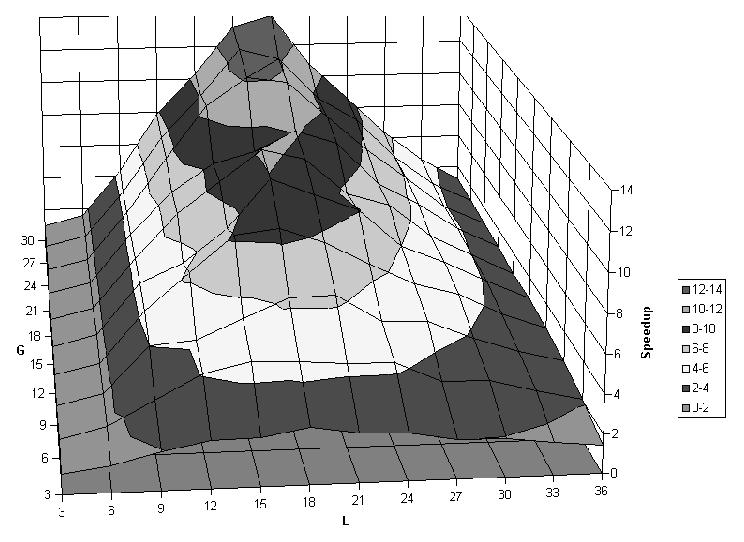
\psfig{file={bfp_depth/ps/q8spdup.ps}} \hfill}
\caption{Speedup for 8-queens benchmark for $G=1\ldots 30$ and $L=1\ldots 36$.}
\vspace{5mm}
\label{q8_3d}
\end{figure}

\begin{figure}[htb]
\vspace{5mm} \hbox to \hsize{\hfill 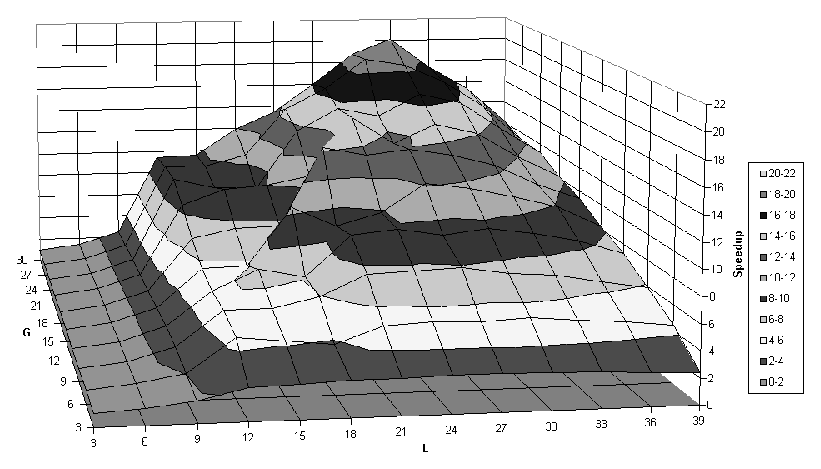
\psfig{file={bfp_depth/ps/q10spdup.ps}} \hfill}
\caption{Speedup for 10-queens benchmark for $G=1\ldots 30$ and $L=1\ldots 39$.}
\vspace{5mm}
\label{q10_3d}
\end{figure}

\begin{figure}[htb]
\vspace{5mm} \hbox to \hsize{\hfill 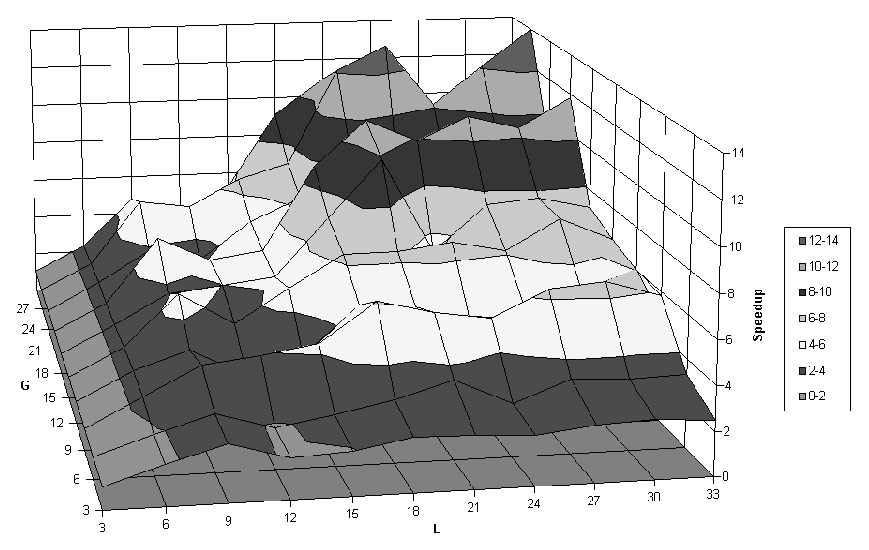
\psfig{file={bfp_depth/ps/pentsp.ps}} \hfill}
\caption{Speedup for Pentominoes benchmark for $G=1\ldots 30$ and $L=1\ldots 33$.}
\vspace{5mm}
\label{pent_3d}
\end{figure}

\subsection{Fixed versus demand-based oracle allocation}
%%%%%%%%%%%%
\label{demand_alloc}

Table \ref{pent_12_runtimes} gives the sorted runtimes for each processor in a
12-processor configuration for the solution of the Pentominoes problem with
a depth limit $L=21$.  The runtimes range from 2874 milliseconds for
path processor 0, through to 91939 milliseconds for path processor 3.

The total runtimes vary because the simple fixed allocation of one twelfth of the
848 oracles at $L=21$ to each path processor (70 or 71 oracles to each) takes place
without any consideration of the size of the subtree beneath each oracle.  The total
workload is thus randomly distributed across the 12 path processors, resulting in an
uneven distribution.  As was discussed in Sections \ref{orc_discovery} and
\ref{work_estimation}, the distribution
is particularly sensitive to the presence of large 'outlier' oracles, and in the
case of the Pentominoes problem is determined by the allocation of the largest 7\% of
the oracles representing 95\% of the work.

The fixed allocation algorithm where the $848$ oracles in the Pentominoes problem are
divided equally and permanently among the available path processors is particularly
simplistic.  If we take the case discussed above with $G=12$ and each path processor
receiving $70$ oracles, a path processor may execute one or more large outlier oracles
at an early stage in its execution with many oracles still to be executed. At this stage
other path processors may already be idle, but the simple algorithm does not permit the
reassignment of the remaining oracles to the idle path processors.  This issue can be
mitigated without the use of a work estimation function, as is demonstrated by the
demand based algorithm discussed below.

Without an effective work estimation function for the oracles, the parallel
performance might be improved with the use of a demand-based allocation algorithm
rather than the current fixed distribution.  The demand algorithm would operate as
follows:
\begin{enumerate}
\item{The breadth-first partitioning phase would execute as before, generating
  a number $S$ of open oracles at the depth limit $L$, forming an ordered list of
  oracles numbered $0\ldots S-1$.}
\item{Each of the $G$ available path processors with processor numbers $N=0$ through $N=G-1$ would
  be assigned an initial oracle with the same number as the path processor number.}
\item{On completion of the search of the subtree beneath the initially assigned oracle, each
  path processor will request an additional oracle from the control processor.  The path
  processor continues to request oracles after each assigned oracle is completed.
  Solutions found while processing an assigned oracle are returned to the control processor
  (or logged locally) and processing continues.}
\item{The control processor will allocate the remaining oracles to requesting path processors in
  the order of the incoming requests, until all the oracles have been allocated.}
\item{The path processors become idle on completion of an assigned oracle when the control
  processor indicates no further oracles are available.}
\end{enumerate}

For the Pentominoes problem with $G=12$ and $L=21$, the allocation of the $848$ oracles on
a demand basis can be simulated to result in the runtimes given in Table \ref{pent_demand0}.

\begin{table}[htb]
{\small
\begin{tabular}{| r | r | r |}
\hline
\textbf{Path Processor} & \textbf{Oracle count} & \textbf{Runtime} \\
\hline
10 & 95  & 33752 \\
6  & 71  & 34007 \\
0  & 29  & 35205 \\
1  & 44  & 35342 \\
4  & 69  & 35776 \\
8  & 43  & 36268 \\
2  & 79  & 36789 \\
3  & 103 & 40169 \\
7  & 70  & 41557 \\
5  & 79  & 42527 \\
11 & 105 & 42812 \\
9  & 61  & 43443 \\
\hline
\end{tabular}
}
\caption{Runtimes of each path processor for Pentominoes $G=12$, $L=21$ using demand allocation
  with no retrieval delay.}
\label{pent_demand0}
\end{table}

Table \ref{pent_demand0} shows that the work is allocated more evenly than with the simple
fixed allocation algorithm,  with a widely varying number of oracles being assigned to
each path processor.  Path processor number 9 has the longest runtime, resulting in a
speedup over the single-cpu case of $445959/43443$, or $10.3$, an improvement on the speedup of
$4.8$ with the fixed allocation.

However, Table \ref{pent_demand0} represents the maximum improvement over the fixed allocation
algorithm as the overhead associated with each request for an oracle has been set at zero
milliseconds.  The demand allocation algorithm is sensitive to the communications delay
associated with every request for an oracle, as can be shown with the Pentominoes problem for
a range of depth limits with $G=30$.

Figure \ref{pent_cut_c_G_30_spdup} shows the speedup achieved by PrologPF for the Pentominoes
problem for values of the depth limit $L=1\ldots 30$ and $G=30$ using the fixed oracle allocation
algorithm.  The graph also shows the calculated speedup performance for a demand-based
oracle allocation algorithm with oracle retrieval delays of $0$, $25$ and $250$
milliseconds.

At each value of the depth limit $L$, the number of oracles generated $S$ and the time
taken for this initial oracle discovery phase are given in table \ref{pent_L_S_BFtime}.

\begin{table}[htb]
{\small
\begin{tabular}{| r | r | r |}
\hline
\textbf{Depth Limit $L$} & \textbf{Oracle count $S$} & \textbf{BFtime} \\
\hline
1  &    1 & 0 \\
3  &    2 & 4 \\
6  &   12 & 4 \\
9  &   44 & 12 \\
12 &  134 & 58 \\
15 &  268 & 156 \\
18 &  472 & 332 \\
21 &  848 & 672 \\
24 & 1410 & 1261 \\
27 & 2256 & 2281 \\
30 & 3396 & 3702 \\
\hline
\end{tabular}
}
\caption{Oracle count $S$ and initial oracle discovery time (BFtime) for Pentominoes
  problem with $L=1\ldots 30$.}
\label{pent_L_S_BFtime}
\end{table}

With reference to Figure \ref{pent_cut_c_G_30_spdup}, the demand-based oracle allocation
algorithm with the retrieval delay of zero or $25$ milliseconds outperforms the fixed
allocation algorithm used by PrologPF for all values of $L$.  With an oracle retrieval
delay of $250$ milliseconds, the overhead of the demand-based algorithm increases with the
number of oracles $S$.  Table \ref{pent_L_S_BFtime} shows that for $L=30$, the number of
oracles discovered $S=3396$.  For $G=30$ at least one processor will be allocated at
least $3396/30$, or $113$ oracles.  
The time taken to retrieve these $113$ oracles places an upper limit on the possible
speedup with the demand-based allocation algorithm.
With a retrieval delay of $250$ milliseconds, the
cumulative delay associated with the allocation of the oracles will be $113\times 250$,
or $28250$ milliseconds, such that at least one path processor will take at least this amount
of time to complete, so the speedup is limited by the retrieval delay to a maximum of
the single-cpu time divided by $28250$, or $15.8$.  In practice the oracles also have
a subtree search time, such that the speedup curve peaks for a value of $L$ with an optimal
balance of granularity of work under the discovered oracles with a sufficiently small oracle
count $S$ to mitigate the retrieval overhead.  The graph in Figure \ref{pent_cut_c_G_30_spdup}
shows this balance to be optimal with $L=18$ for an oracle count $S=472$.

\subsection{Work splitting}
%%%%%%%%%%%%
\label{bfp_work_splitting}

After the initial breadth-first partitioning phase in which the open oracles are
discovered at the selected depth limit $L$,  PrologPF uses a simple fixed allocation
algorithm to assign the oracles to the available path processors.  After this assignment
takes place, with one-time partitioning the path processors search the subtrees of all 
their allocated oracles
and become idle when all this work is completed.  Some path processors will complete
their assigned work and become idle before others.  An example of this behaviour is
illustrated in Table \ref{pent_12_runtimes}, where path processor 0 becomes idle after
only 2827 milliseconds while path processor 3 executes for 91939 milliseconds.

As the parallel performance is determined by the path processor with the highest runtime, a
more balanced distribution of the work will increase the overall speedup.  To balance the
workload in the example discussed, work must be transferred from path processor 3 to
other path processors.

Relative to the fixed allocation of oracles used by PrologPF and DelphiKS, the demand
allocation of oracles discussed in Section \ref{demand_alloc} represents a dynamic
distribution of the workload.  In effect the work that would otherwise reside in the
pool of oracles assigned to processor 3 is collected by other path processors as they
become idle.  However, the 'outlier' oracles discussed in Section \ref{orc_discovery}
represent an additional problem, in that a path processor will proceed without
interruption to search the entire subtree beneath any given oracle.

This issue is more significant the more imbalanced the work between
the $S$ discovered open oracles at the selected depth limit $L$.
Empirically, the imbalance in workload between the discovered oracles
become worse the smaller the depth limit and the fewer the discovered
oracles.

The issue of work splitting is illustrated in Figure \ref{work_split_figure}.

\begin{figure}[htb]
\vspace{5mm} \hbox to \hsize{\hfill \psfig{file={bfp_depth/ps/work_split_figure.ps}} \hfill}
\caption{Work splitting at busy path processor.}
\vspace{5mm}
\label{work_split_figure}
\end{figure}

In Figure \ref{work_split_figure} the initial depth limit has been set at L, and the
illustrated path processor $N$ has been assigned the open oracles A, B, C, D and E.
The figure illustrates the situation at some point while path processor $N$ is
searching the subtree of oracle C, having completed oracles A and B.  At this
point other path processors have completed all their oracles and have become idle.
The parallel performance of the system may be improved if the remaining work of
path processor $N$ can be assigned to the idle path processors.  With the architecture
of the Delphi machine, the remaining work can be categorised as being of two types:
\begin{enumerate}
\item{The oracles D and E represent subtrees yet to be searched.}
\item{Path processor $N$ is currently at point X in its search of the subtree beneath
  oracle C, proceeding with the standard Prolog depth-first left-to-right search.  The
  portion of the subtree under oracle C to the right of X remains to be searched.}
\end{enumerate}

For the first case, the reassignment of the work of the remaining oracles can be
effected by allocating the remaining oracles D and E to two idle processors.

The second case, in which path processor $N$ has partially searched the subtree
under oracle C to arrive at point X, may require more complex treatment
involving an incremental breadth-first partitioning phase starting from oracle C
rather than the root of the problem search tree.  This phase will discover the
open oracles C1, C2, C3 and C4 at the new depth limit L1.

Then the simplest approach may be to discard the work already performed
by path processor $N$, and to add that path processor to the pool of idle path
processors for the oracle reassignment.  Those processors then search the subtrees
below oracles C1, C2, C3 and C4 in parallel.

An issue arises if solutions have been found by path processor $N$ and returned
to the control processor.  Further solutions found by the group of processors
assigned oracles C1, C2, C3 and C4 may be duplicates of those already returned.
If the previous search to position X
by path processor $N$ is ignored, then the solutions returned must be labelled with
their associated oracle, such that subsequent duplicates can be discarded.  The use
of an oracle to uniquely identify a point in the search tree provides a powerful
mechanism to label any solution with a unique identifier.  In problems requiring
only one solution, or where duplicate solutions are acceptable or ignored, the
transmission of the oracle with the solution is no longer necessary.

A more complex approach to reassigning the work of path processor $N$ beneath oracle
C in Figure \ref{work_split_figure} can take advantage of the
availability of the current oracle in path processor $N$ referring to point X at the
time of interruption.  If the incremental partitioning depth L1 is smaller than
the current depth of X, then the oracles found at L1 have the following characteristics:
\begin{enumerate}
\item{One of the open oracles discovered at the incremental depth limit L1 
 (C1, C2, C3 or C4) will form a prefix of
  the oracle to X.  This is necessary
  because if X is a valid point in the search space then all oracles representing every
  choice point up to X \textit{must} have further open branches to include X, and 
  cannot be closed oracles representing success or failure.  For the following
  discussion this oracle will be called C$_x$.}
\item{All oracles at the incremental depth limit L1 which are numerically smaller than
  the oracle formed from the first L1 indexes in the oracle leading to X have already
  been fully searched by path processor $N$.  This is true because the oracle indexes are
  ordered in the same order as the textual sequence of the associated clauses, and the
  search order used by PrologPF is the same as that of Prolog, namely top-down.}
\end{enumerate}

If further refinement is required, the subtree referred to by oracle C$_x$ (see above) can
be further partitioned at an incremental depth L2 to generate additional open oracles.
The same reasoning can be used as above to identify the single oracle within this ordered
list which includes X, such that all open oracles to the right of that oracle can be
assigned to idle path processors.

Chapter \ref{sok} builds upon a modified breadth-first partitioning technique to support
work-splitting in PrologPF.

%%%%%%%%%%%%%%%%%%%%%%%%%%%%%%%%%%%%%%%%%%%%%%%%%%%%%%%%%%%%%%%%%%
\section{Breadth-first partitioning versus stream-AND parallelism} %
%%%%%%%%%%%%%%%%%%%%%%%%%%%%%%%%%%%%%%%%%%%%%%%%%%%%%%%%%%%%%%%%%%
\label{bfp_stream_and}

Stream-AND parallelism in logic programming relies upon the treatment of
certain relations as \textit{producers} and other relations as \textit{consumers}.
Newmarch provides a tutorial introduction to stream-AND parallelism
in \cite{New90} Chapter 10, and the
technique is reviewed in this dissertation in
Chapter \ref{background} Section \ref{and_parallelism_section}.

A conjunctive goal such as \texttt{member(X,Biglist), factorial(X,Y)} can be
viewed as a pair of connected parallel processes \texttt{member} and
\texttt{factorial}.  The \texttt{member} process generates values and sends them
to the \texttt{factorial} process, which in turn produces the associated sequence
of factorials.  The parallel speedup arises from the fact that the \texttt{member}
process can be working on the production of the next value while the \texttt{factorial}
process is still working on the previous value.

The breadth-first partitioning scheduling strategy can produce comparable benefits
when the producer process involves relatively little work.
This can be illustrated with
a sample tree for a \texttt{member/factorial} query with the program listed below.
The search tree for the following \texttt{member/fact} program is given in
Figure \ref{stream_and}.

\begin{verbatim}
member(X,[X|_]).
member(X,[_|Y]) :- member(X,Y).

fact(1,1).
fact(X,F) :- X > 1, X1 is X-1, fact(X1,F1), F is X*F1.

:- member(X,[4,3,2,1]), fact(X,Y).
\end{verbatim}

\begin{figure}[htbp]
\vspace{5mm} \hbox to \hsize{\hfill \psfig{file={bfp_depth/ps/stream_and.ps}} \hfill}
\caption{Search tree for \texttt{member/fact} program.}
\vspace{5mm}
\label{stream_and}
\end{figure}

At the selected depth limit L a number of oracles are discovered which can be passed
to available path processors for execution.  These path processors will recompute the
value of \texttt{X} generated by the \texttt{member} relation by following the
assigned oracle.  Following an oracle is an efficient operation which takes a time
proportional to the length of the oracle, L.  The reconstructed value of \texttt{X}
is then passed to the \texttt{fact} relation for the relatively lengthy computation.
The approach is most effective if the subsequent computation is much greater than
the initial work generating and following the open oracles, and the technique is
suited to \textit{generate-and-test} programs where the \textit{test} is complex.

%%%%%%%%%%%%%%%%%%%%%%%
\section{Conclusions} %
%%%%%%%%%%%%%%%%%%%%%%%

The benchmark programs used to evaluate the pure Prolog performance of PrologPF
have sufficient OR-parallelism to provide useful results in tests with 1 to
30 path processors\footnote{The experimental system at Cambridge was generally limited during
this research to 30 processors}.
Execution of the programs has illustrated issues relating to
the overall size of the selected problem, the use of the breadth-first partitioning
scheduling algorithm, and the selection of the depth limit used in that
scheduling algorithm.

PrologPF has an efficient implementation with the use of simple oracle
management primitives \texttt{o\_{}build} and \texttt{o\_{}follow} 
written in 'C' combined with a standard Prolog compiler.  Similar
primitives can be implemented in Prolog giving a flexible system
suitable for evaluation of the use of oracles with an acceptable
performance penalty.  The PrologPF overhead relative to the use of the standard compiler
in a single-cpu environment for the test programs was 9 to 19\%.

The breadth-first partitioning algorithm provides a means of allocating the work
to a number of available path processors with no subsequent communication after
the initial assignment of the problem.  The optimal selection of the depth limit
for the breadth-first partitioning strategy has a significant impact on the
effectiveness of the subsequent parallelisation, with the fixed one-time work
allocation algorithm resulting in an uneven utilisation of the path processors.
The utilisation of the path processors would be more even if the breadth-first
oracle discovery technique were complimented with a demand-based allocation
algorithm and work splitting of large oracles during their execution if other path
processors are idle.

PrologPF with its breadth-first partitioning algorithm provides similar parallelisation
benefits to those obtained with stream-AND parallelism for
generate-and-test programs in which the
generation procedure is relatively lightweight.

%%%%%%%%%%%%%%%%%%%
\section{Summary} %
%%%%%%%%%%%%%%%%%%%

Three OR-parallel pure Prolog benchmarks have been used to 
investigate the effectiveness of the parallelisation techniques used in PrologPF:
\begin{description}
\item[8-queens: ]{the chess-based problem of fitting eight queens onto an
  eight-by-eight chessboard with none attacking any other.}
\item[10-queens: ]{the same problem with ten queens and a ten-by-ten chessboard.}
\item[Pentominoes: ]{the problem of fitting twelve defined geometric shapes onto
  a three-by-twenty board.}
\end{description}
The programs selected have been used to:
\begin{enumerate}
\item{Assess the speedup provided by PrologPF for the execution of each problem on
  a range of distributed systems with 1 to 30 processors.}
\item{Compare the performance of PrologPF with previous implementations of the
  Delphi machine.}
\item{Compare the performance of PrologPF and previous Delphi implementations with
  the single-cpu performance of other compilers.}
\item{Investigate the overhead of the partitioning time for a range of values of
  the depth limit parameter of the breadth-first partitioning algorithm.}
\item{Investigate the impact of the random distribution of the workload beneath the
  typical range of discovered open oracles.}
\end{enumerate}

The earlier implementation of a Prolog system using oracles, DelphiKS, utilised
an extended Warren Abstract Machine \cite{War83} with additional instructions for
oracle manipulation.  A prototype version of PrologPF uses Prolog data structures
to hold the oracles, with Prolog procedures to create and interpret the
structures.  The final version of PrologPF uses similar procedures written in 'C'
with the oracles held in 'C' arrays for a faster execution.  Each system has produced
compiled binaries suitable for parallel execution on a distributed system of common Unix
workstations.

PrologPF is based upon the 'wamcc' Prolog compiler \cite{CD95}.  The following table
compares the single-cpu performance of DelphiKS, PrologPF with Prolog oracle primitives,
PrologPF with C primitives, wamcc, and SICStus Prolog Version 3 (compactcode)
on the same DECStation 3100.
The figures are calculated from the geometric mean of the results of the three
benchmarks used, and are normalised against wamcc.

\begin{table}[htb]
{\small
\begin{tabular}{| r | r | r | r | r |}
\hline
 & & & & \\[2mm]
\textbf{DelphiKS} & \textbf{PrologPF(Prolog)} & \textbf{PrologPF(C)} & \textbf{wamcc} & \textbf{SICStus} \\
\hline
 19.8 & 3.95 & 1.15 & 1.00 & 1.61 \\
\hline
\end{tabular}
}
\caption{Single cpu runtime ratios.}
\label{single_cpu_ratios}
\end{table}

In this analysis PrologPF uses a breadth-first partitioning strategy, in which an initial phase of
execution proceeds in the normal Prolog depth-first left-to-right manner, but is limited
to a selected AND-OR depth.  During execution, PrologPF maintains a list of the indexes of
each clause leading to the current position in the search, this list being the current
\textit{oracle}.  Each time the depth limit is reached in the initial phase, the current
oracle is recorded on the \textit{oracle stack}.  On completion of the initial phase
of execution, the oracles on the oracle stack are assigned to the available path processors
for re-execution in a second phase in which the subtree beneath each can be searched.

For the 8-queens problem, PrologPF achieved a maximum speedup with 30 processors of 13.5.
On the same distributed system the speedup achieved for the 10-queens problem was 18.5 and
for the Pentominoes problem was 10.8.  The runtime for the 8-queens problem was
reduced from 1.9 seconds to 141 milliseconds, the 10-queens problem from 46.5 seconds to
2.5 seconds, and the Pentominoes problem from 446 seconds to 41.5 seconds.

The benchmark programs were used to investigate the characteristics of the breadth-first
partitioning strategy.  In general, the actual speedups achieved were less than the
number of available path processors.  The analysis of the actual performance of
the benchmarks clarified the issues involved, suggesting improvements to the technique.

The issues can be summarised as follows:
\begin{enumerate}
\item{The initial breadth-first partitioning phase of execution is performed sequentially,
  without benefit of parallel speedup.  The time taken to generate the open oracles
  during this phase places an upper bound on the overall speedup.  This issue is most
  apparent in programs with relatively small search trees, as the initial breadth-first
  phase can represent an appreciable proportion of the overall execution.}
\item{After the open oracles have been generated and allocated, each path processor will
  follow each of its assigned oracles to arrive at the associated subtree.  Following
  an assigned oracle represents a recomputation of that section of the search space.  If
  a large number of oracles is generated, each of a significant length (the depth limit
  was relatively deep) then this recomputation overhead may be significant.}
\item{With a fixed one-time allocation of oracles to the available path processors without
  any consideration of the work beneath each oracle, the work to the path processors may
  be imbalanced, leading to a range of total runtimes for the path processors.  As the
  parallel performance for an all-solutions problem is determined by the longest running
  path processor, this leads to a reduction in overall speedup.}
\item{The analysis of the benchmarks shows that the subtrees represented by
  the oracles discovered at the depth limit refer to subtrees containing widely differing
  amounts of work.  In many cases, the majority of the oracles refer to relatively small
  subtrees, while a minority refer to a small number of very large subtrees.  Not only
  all the oracles allocated at the end of the first breadth-first partitioning phase, but
  the subtree beneath each individual oracle is searched to completion.  Other path
  processors may be idle while one path processor is busy in the search of a very large
  subtree.}
\end{enumerate}

The analysis of these issues suggests a number of improvements needing further work:
\begin{itemize}
\item{The time spent in the initial breadth-first partitioning phase is a more
  significant issue for small problems, becoming less significant as the problem size
  increases.  This issue might be ignored for large problems, or compile-time analysis
  might be used to optimise the strategy for smaller problems such as 8-queens.}
\item{The recomputation overhead associated with following oracles is very low with the
  breadth-first partitioning strategy, as the time spent following the allocated oracles
  to arrive at the designated subtree is much lower than the time spent searching the
  subtrees.  For this overhead to be minimised a good technique is needed to generate
  as many oracles with non-trivial subtrees as possible.  The automatic partitioning
  strategy \cite{Kle91, Sar95} was greatly impacted by this issue,  and breath-first
  partitioning improves the situation by generating a much larger pool of open oracles.}
\item{The fixed allocation of the oracles after the initial breadth-first partitioning
  phase minimises the subsequent communication requirements, but leads to a significant
  imbalance of the workload.  The workload can be much better balanced with a demand-based
  strategy, in which the path processors request additional oracles on completion of the
  search of each assigned oracle.  A trade-off is made of the workload balancing against
  the communications requirements.}
\item{The presence of large outlier oracles in the pool discovered at the
  selected depth limit implies that work splitting is required to interrupt the execution
  of a busy processor to re-partition the work associated with the large oracle. One
  approach is to re-use the breadth-first partitioning strategy within
  the subtree represented by the large oracle.  The ordering of the clause indexes combined
  with the Prolog strict top-down left-to-right search means that some optimisations can
  be applied to take advantage of the search within the subtree already performed by the
  busy path processor.  These enhancements are discussed in Chapter \ref{sok}.}
\end{itemize}

For some problems, PrologPF with the breadth-first partitioning strategy provides similar
parallel behaviour to that obtained with stream-AND parallelism.  The producer-consumer
model in stream-AND parallelism is replaced in PrologPF with a recomputation technique
for the generation of the 'produced' values.  The techniques are comparable in
efficiency  if the computational requirements of the
producer procedure are relatively low.

In general, PrologPF provides effective speedup for many Prolog programs on a
distributed network of general-purpose workstations.  The technique is simple, and
suited to an environment where many workstations are available.  No special programming
techniques are required, and the use of oracles allows speedy recovery in the event
of an individual workstation failure.


